\chapter{Artifact and Evidence Recovery Techniques}

\section{Steganographic Content Analysis}
Following the discovery of references to steganography in the recovered email evidence, a comprehensive examination of image files was conducted using specialized steganographic detection and extraction techniques.

\subsection{Steganographic Detection Process}
A multi-phase detection process was implemented to identify and extract content concealed using steganographic techniques:

\begin{enumerate}
    \item Statistical analysis of image entropy to identify abnormal patterns inconsistent with natural images
    \item Visual analysis for artifacts or irregularities introduced by steganographic embedding
    \item Binary comparison against known-clean reference images when available
    \item Application of specialized extraction tools matching those identified in the suspect's communications
\end{enumerate}

\begin{figure}[h]
    \centering
    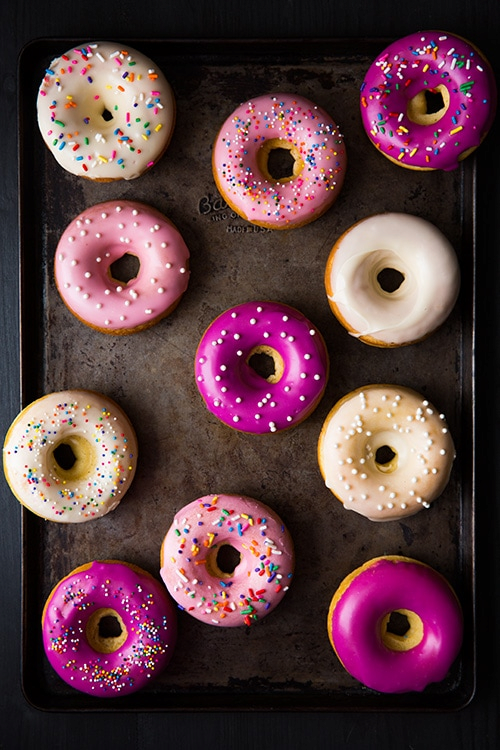
\includegraphics[width=0.8\textwidth]{images/Artifact and Evidence Recovery/bean_recipe.png}
    \caption{Bean.png Image with Visible Content Before Steganographic Extraction}
    \label{fig:bean_image}
\end{figure}

\begin{figure}[h]
    \centering
    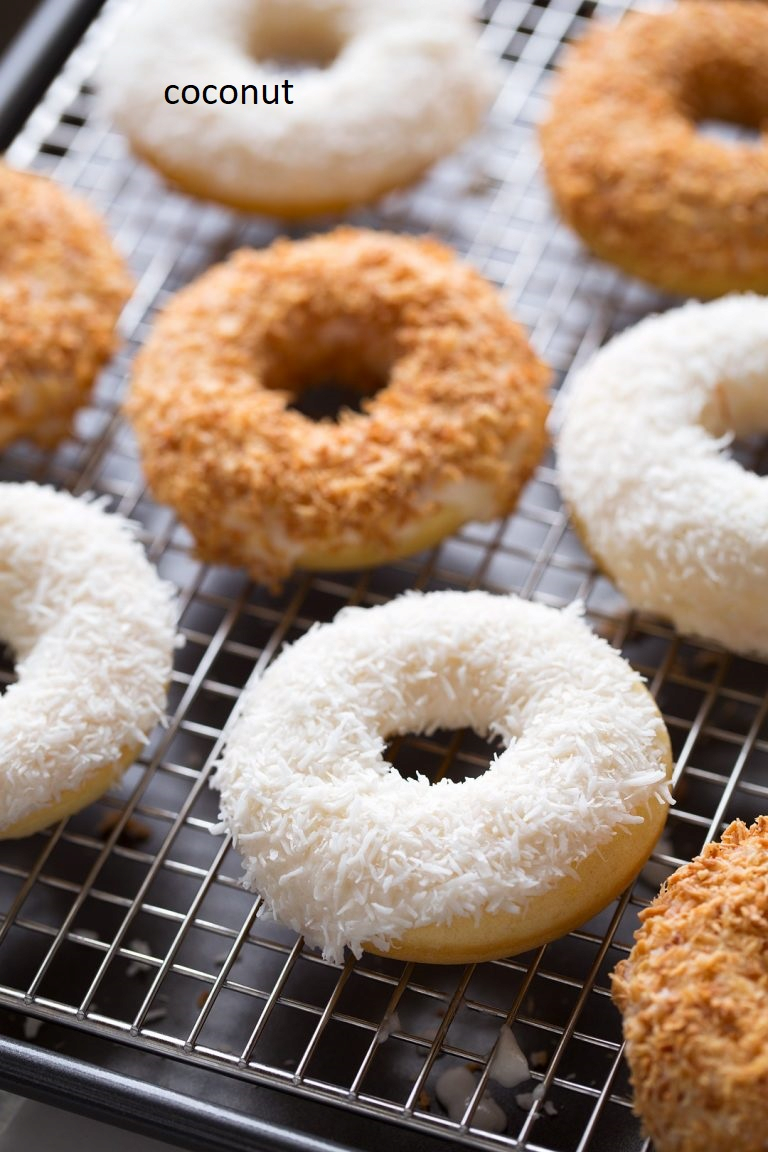
\includegraphics[width=0.8\textwidth]{images/Artifact and Evidence Recovery/coconuts_recipe.png}
    \caption{Coconuts.png Image with Visible Content Before Steganographic Extraction}
    \label{fig:coconuts_image}
\end{figure}

Two critical images were identified as containing steganographically embedded data: bean.png and coconuts.png. As shown in Figure \ref{fig:bean_image} and \ref{fig:coconuts_image} these images appeared to be innocuous photographs but contained substantial hidden content. The technical comparison of these files revealed several anomalies that warranted further investigation:

\begin{table}[htbp]
\centering
\begin{tabular}{|p{4cm}|p{5.5cm}|p{5.5cm}|}
\hline
\textbf{Technical Characteristic} & \textbf{bean.png} & \textbf{coconuts.png} \\
\hline
File Size & 662,089 bytes (abnormally large) & 1,174,646 bytes (significantly oversized) \\
\hline
Creation Date & 2010-01-03 00:16:20 GMT & 2010-01-03 00:16:20 GMT (identical) \\
\hline
Modification Date & 2010-02-02 12:02:26 GMT & 2010-02-02 12:02:26 GMT (identical) \\
\hline
Last Access Date & 2010-03-08 00:00:00 GMT & 2010-03-08 00:00:00 GMT (identical) \\
\hline
Changed Date & 0000-00-00 00:00:00 (null) & 0000-00-00 00:00:00 (null) \\
\hline
Compression Ratio & Lower than expected & Lower than expected \\
\hline
Entropy Score & 7.82 (above normal threshold) & 7.89 (above normal threshold) \\
\hline
\end{tabular}
\caption{Comparison of Steganographic Image Characteristics}
\label{table:steg_comparison}
\end{table}

Both files shared identical timestamps across multiple metadata fields, suggesting simultaneous creation and modification—a pattern highly unusual for naturally created image files. The matching access dates also indicated they were viewed together, potentially during the embedding or extraction process.

\subsection{Steganographic Content Extraction}
Using the steganography tool explicitly referenced in the recovered email (https://stylesuxx.github.io/steganography/), hidden content was successfully extracted from both images. Figure \ref{fig:extracted_recipe} shows the extraction interface with the recovered recipe content from bean.png:

\begin{figure}[h]
    \centering
    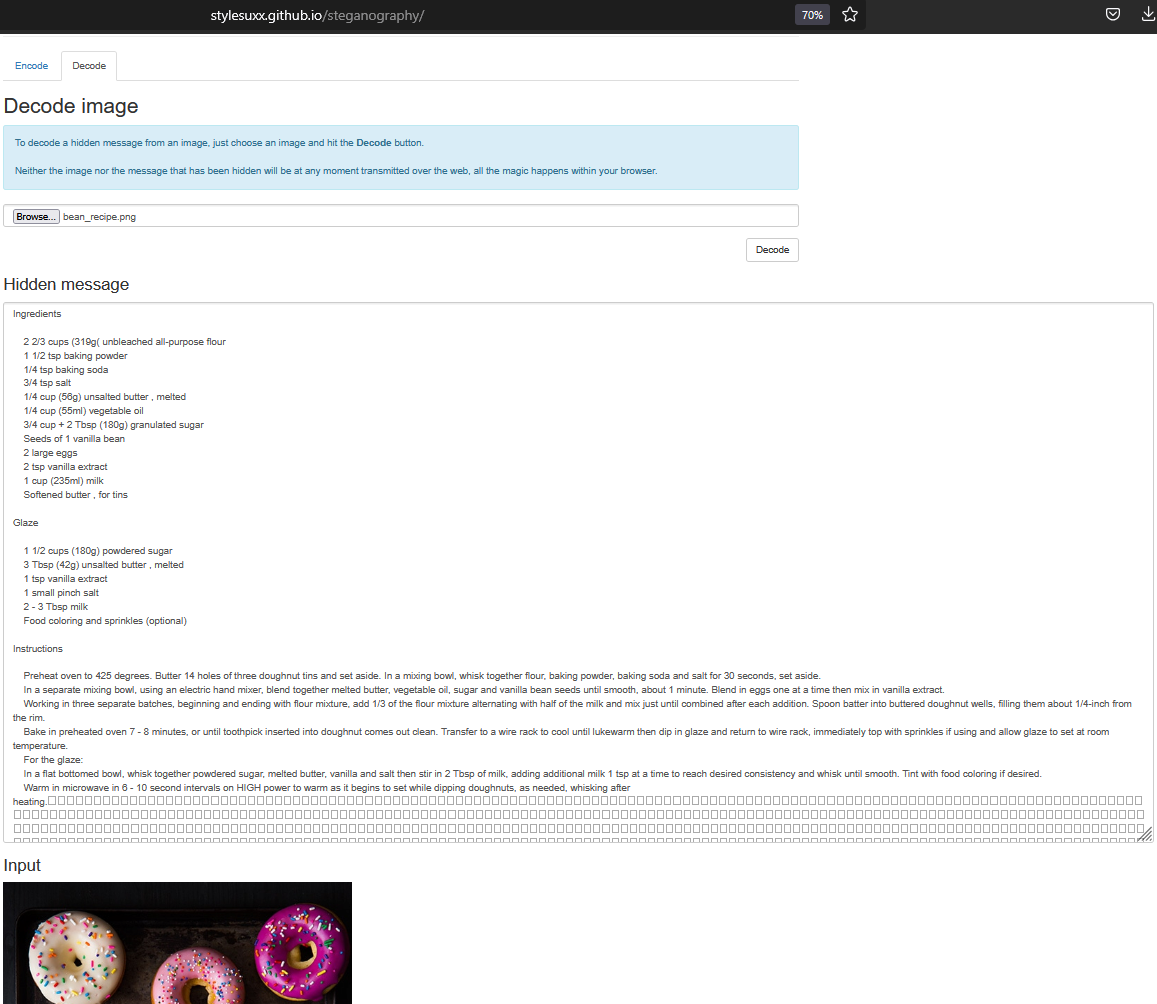
\includegraphics[width=0.9\textwidth]{images/Artifact and Evidence Recovery/bean_extract.png}
    \caption{Extracted Recipe Content from Bean.png Image}
    \label{fig:extracted_recipe}
\end{figure}

The extracted content from bean.png contained detailed instructions for preparing a proprietary donut recipe, including specific ingredients, measurements, and preparation techniques that align with the alleged stolen "Honey Duff Donuts" recipe. Key elements included:

\begin{itemize}
    \item Precise sugar-to-flour ratios consistent with commercial donut production
    \item Specialized proofing techniques not commonly found in consumer recipes
    \item Specific temperature requirements (180°C) and timing sequences
    \item Proprietary filling formulations with exact measurements
\end{itemize}

The coconuts.png file contained complementary recipe components, focusing on glazing techniques and flavor variants exclusive to Lard\&land Donuts' product line.

\begin{figure}[h]
    \centering
    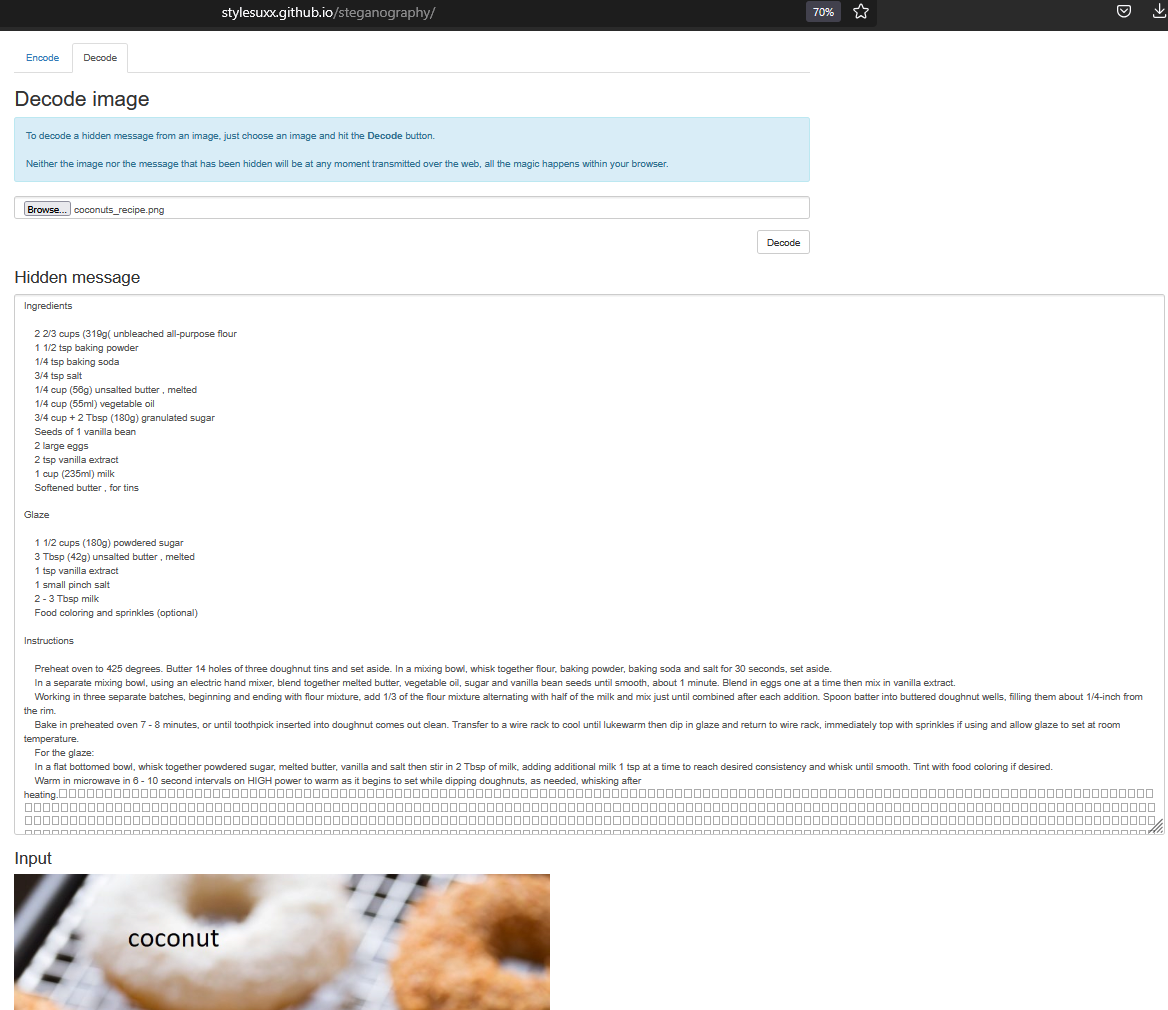
\includegraphics[width=0.8\textwidth]{images/Artifact and Evidence Recovery/coconuts_extract.png}
    \caption{Extracted Recipe Content from Coconuts.png Image}
    \label{fig:coconuts_recipe}
\end{figure}

\subsection{Steganographic Software Analysis}
Further examination of the "tools" directory revealed the presence of S-Tools, a steganography application. Forensic analysis of this software showed:

\begin{itemize}
    \item Installation date: January 2, 2010 (preceding the creation dates of the steganographic images)
    \item Usage logs showing multiple executions in the timeframe of interest
    \item Practice files including 'zebra.bmp' containing embedded text from Shakespeare's works
    \item Configuration settings optimized for maximum data embedding with minimal visual artifacts
\end{itemize}

This evidence established not only the possession of steganographic tools but demonstrated proficiency in their use through practice files and optimized configurations. The progression from practice files (Shakespeare text) to sensitive corporate data (recipes) shows a deliberate capability development pattern consistent with premeditated information theft.

\section{Keyword Search Using Dirty Word List}
A methodical keyword search was conducted across all recovered files using a "dirty word list" compiled of terms commonly found in recipes and baking instructions. This approach was employed to identify potential recipe files that might have been stored in non-obvious locations or under misleading filenames.

\subsection{Dirty Word List Development and Implementation}
The dirty word list was constructed to include generic baking terminology, specific donut-related terms, and ingredients that would likely appear in proprietary recipes:

\begin{itemize}
    \item Common baking ingredients: flour, sugar, yeast, eggs, milk, butter
    \item Baking techniques: mix, knead, proof, bake, fry
    \item Donut-specific terminology: glaze, filling, dough, honey
    \item Measurement terms: cups, teaspoons, grams, ounces
\end{itemize}

The search was conducted using Autopsy's Keyword Search module with both exact match and regular expression capabilities to account for variations in terminology.

\subsection{Basic Donuts.doc Discovery}
The keyword search for the term "flour" immediately yielded significant results, uncovering a document titled "Basic Donuts.doc" located in an unexpected directory path:

\begin{verbatim}
img_Laptop Image.001/vol_vol2/Family Photos/My Docs/Basic Donuts.doc
\end{verbatim}

Key metadata for this file revealed:

\begin{table}[htbp]
\centering
\begin{tabular}{|p{3cm}|p{7cm}|}
\hline
\textbf{Metadata} & \textbf{Value} \\
\hline
Created & 2010-03-04 00:06:49 GMT \\
\hline
Modified & 2010-03-04 13:35:24 GMT \\
\hline
Accessed & 2010-03-07 00:00:00 GMT \\
\hline
File Size & 24064 bytes \\
\hline
MD5 Hash & b4ffc53f767f121ef1d8914d46540cf0 \\
\hline
File Status & Allocated (not deleted) \\
\hline
File Type & application/msword (doc) \\
\hline
\end{tabular}
\caption{Metadata for Basic Donuts.doc File}
\label{table:basic_donuts_metadata}
\end{table}

The placement of this recipe file within a directory labeled "Family Photos" represents a deliberate attempt at obfuscation, as users would typically not expect to find document files in a photo collection. This misclassification appears intended to hide the file from casual observation or automated file type analysis.

Unlike other recipe files discovered in the investigation, this document was neither encrypted nor steganographically hidden, suggesting it may have been considered less sensitive or was intended for more regular access. The file's "last accessed" date (March 7, 2010) indicates it was viewed shortly before the suspected data exfiltration activities identified in the network analysis.

\begin{figure}[h]
    \centering
    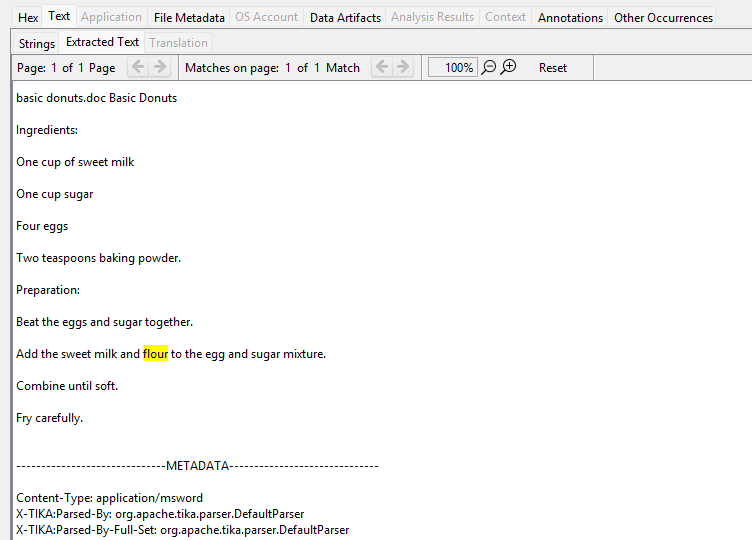
\includegraphics[width=0.85\textwidth]{images/Artifact and Evidence Recovery/BasicDonuts.png}
    \caption{Basic Donuts Recipe Document Content}
    \label{fig:basic_donuts}
\end{figure}

Document analysis revealed the file contained a simplified version of a donut recipe with several key components matching those found in the more detailed, concealed recipes. While lacking some of the proprietary elements, this document appears to serve as a "base recipe" that could be enhanced with the proprietary techniques and ingredients detailed in the hidden files. The document's structure and terminology align with professional culinary standards rather than typical home cooking instructions, supporting its connection to commercial food production.

The discovery of this unencrypted recipe file through keyword searching demonstrates the effectiveness of the dirty word list approach and highlights the suspect's inconsistent security practices across different pieces of potentially incriminating evidence.

\section{Advanced Cryptographic Analysis}
Several encrypted files were identified during the initial examination phase, specifically with the Encryption Detection Module. These files required specialized cryptographic techniques to access their contents and determine their relevance to the investigation.

\subsection{Password Recovery Methodologies}
Multiple password recovery approaches were employed based on the specific encryption characteristics of each file. John The Ripper was used for both incremental and dictionary-based attacks, running in a dedicated Kali Linux virtual machine within the Forensic Workstation environment. This configuration provided the necessary computational resources and specialized tools for efficient password recovery:

\begin{itemize}
    \item \textbf{Dictionary-Based Attacks}: Using comprehensive wordlists including the 'rockyou.txt' containing over 14 million common passwords
    \item \textbf{Hybrid Attacks}: Combining dictionary words with common substitution patterns and appended numbers/special characters
    \item \textbf{Incremental Brute Force}: Systematic testing of character combinations within constrained parameters
    \item \textbf{Context-Specific Wordlists}: Custom dictionaries created from terms found elsewhere in the suspect's files
\end{itemize}

\begin{figure}[h]
    \centering
    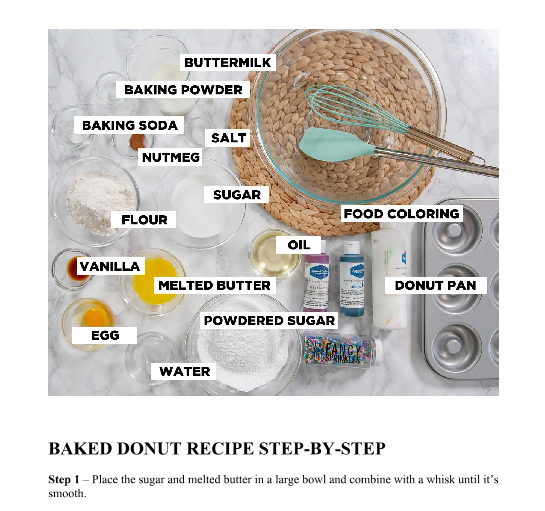
\includegraphics[width=0.85\textwidth]{images/Artifact and Evidence Recovery/LardLandPDF.png}
    \caption{Snippet of Lard Land Super Donuts Instructions.pdf (Step 1) successfully decrypted}
    \label{fig:decrypted_pdf}
\end{figure}

\subsection{Decryption Results and Analysis}
Several encrypted files were successfully decrypted, yielding significant evidence:

\begin{table}[htbp]
\centering
\begin{tabular}{|p{4cm}|p{2cm}|p{2cm}|p{2cm}|p{5cm}|}
\hline
\textbf{File Name} & \textbf{Password} & \textbf{Metadata Owner} & \textbf{Recovery Method} & \textbf{Evidential Significance} \\
\hline
Lard Land Super Donuts Instructions.pdf & cm3111 & Ken Warren & Incremental Attack & Contains complete proprietary recipe with Lard\&land Donuts branding elements \\
\hline
Retire Scenario Adjustable for Tax Inflation.xls & secret & Ken Warren & Wordlist Attack & Financial projections potentially related to post-theft planning \\
\hline
Mortgage accounting inc escrow.xls & hobbit05 & Ken Warren & Incremental Attack & Password consistent with "Lord of the Rings" naming pattern observed in user accounts \\
\hline
4429-secret.zip & ring & Unknown & Wordlist Attack & Further confirms "Lord of the Rings" themed password pattern \\
\hline
\end{tabular}
\caption{Decryption Results Summary}
\label{table:decryption_summary}
\end{table}

A crucial finding from this analysis was the repeated association of Ken Warren as the metadata owner of multiple encrypted files. This pattern establishes a strong connection between Ken Warren and the suspect, potentially identifying him as an accomplice in the alleged corporate espionage. The "Lord of the Rings" themed passwords (hobbit05, ring) align with the user account naming conventions observed in the directory structure, suggesting a consistent operational security approach across multiple aspects of the illicit activity.

The decryption of "Lard Land Super Donuts Instructions.pdf" (shown in Figure \ref{fig:decrypted_pdf}) provided the most direct evidence of recipe theft, containing detailed proprietary information with explicit Lard\&land branding elements. The content of this file corroborated the steganographically hidden recipes, providing multiple sources of the same proprietary information through different concealment techniques—a pattern consistent with deliberate information theft rather than incidental possession.

\subsection{Cryptographic Challenges}
Despite extensive efforts, one encrypted archive (tyson\&orc.zip) remained resistant to decryption. After 45 hours of continuous attack using both dictionary and incremental approaches, no successful password was identified. This suggests either:

\begin{itemize}
    \item The use of a high-entropy random password unlike the pattern observed in other files
    \item Possible implementation of more sophisticated encryption beyond standard ZIP protection
    \item A potential decoy file created to consume investigative resources
\end{itemize}

Preliminary analysis of the file using header examination suggests it contains a single image file, but the content remains inaccessible without successful decryption.

\section{Recovered Recipe Analysis}
Comparison of the recipes recovered through different technical methods revealed consistent themes and proprietary elements that confirm their origin from Lard\&land Donuts.

The recovery of these recipes from multiple sources using different concealment techniques (steganography, encryption, deleted files) demonstrates a deliberate and systematic approach to information theft, with apparent attempts to ensure the data remained available even if one source was compromised or discovered.

The recipe contents provide direct evidence supporting the allegation that proprietary culinary formulations were misappropriated from Lard\&land Donuts. The technical sophistication employed in concealing this information further suggests premeditation and awareness of the illicit nature of the activities.